\documentclass[12pt]{article}

\usepackage{sbc-template}

\usepackage{graphicx,url}

%\usepackage[brazil]{babel}
\usepackage[utf8]{inputenc}

\usepackage[T1]{fontenc}
\usepackage{amsmath}
\usepackage{hyperref} 

\usepackage{listings}

% Declare problematic Unicode characters
\DeclareUnicodeCharacter{2248}{$\approx$} % U+2248 is the approximation symbol '≈'

\sloppy

\title{Prompt Engineering for Explainable Driver Behavior Analysis Using Telemetry Data}

\author{Isaac M. Oliveira\inst{1} Dr. Rafael S. Parpinelli\inst{1}}

\address{Department of Computing -- Santa Catarina State University (UDESC) -- Joinville -- SC -- Brazil\\\email{rafael.parpinelli@udesc.br, isaac.oliveira@edu.udesc.br}}

\begin{document}

\maketitle

\begin{abstract}
This paper proposes a system for analyzing driver behavior using telemetry data and prompt engineering techniques. Built with Python (Dash and Plotly), the system computes severity scores for events such as speeding and harsh braking. A \textbf{LLM} (Google Gemini) serves as a \textbf{Virtual Driving Instructor}, generating feedback in natural language. The prompt design combines techniques of \textbf{XML structure}, \textbf{Persona}, \textbf{Constitutional AI}, \textbf{Chain-of-Thought}, and \textbf{self-correction}. Based on the literature of \textbf{XAI}, \textbf{DSS}, and \textbf{HCI}, the system improves explainability and user trust.
\end{abstract}

\section{Introduction}

Traffic safety and fleet efficiency fundamentally depend on driver behavior. Telemetry systems today record large amounts of driving data – offering an opportunity to identify risky behaviors and instruct drivers. In practice, however, fleet managers often have difficulty translating telemetric data into actionable feedback for drivers. Traditional feedback mechanisms (e.g., numerical risk scores or incident maps) are not always intuitive or motivating for drivers. Research shows that drivers prefer textual explanations of their performance that provide concrete advice, rather than abstract scores or charts. There is a clear need for explanatory reports that bridge the gap between raw sensor data and human understanding, thereby promoting safer and more efficient driving.

At the same time, recent advances in Large Language Models (LLMs) have enabled AI systems to generate fluent, contextualized text. LLMs, when properly guided, can serve as natural language decision-support interfaces that explain to users insights derived from data. In safety-critical domains such as driving, explainable AI is crucial for user trust and adoption. However, using LLMs for telemetry data analysis presents challenges: the model must remain faithful to the data, adopt an appropriate tone (for example, instructive rather than scolding), and avoid ambiguity or hallucinations. These challenges motivate the use of Prompt Engineering – the craft of designing input prompts and interaction strategies to shape an LLM’s outputs.

This paper proposes an approach that combines telemetry-based driver behavior analysis with advanced prompt engineering techniques to produce easily understandable explanations for drivers. A web application was developed that receives driving data (CSV files of recorded violations) and computes a Gravity Score (severity index) for each event based on configurable business rules. The system includes a “Virtual Instructor” module powered by an LLM, which generates a personalized driver performance report from the analyzed data. To ensure that these AI-generated reports are accurate, constructive, and easy to analyze, a structured prompt was designed with an expert persona, ethical principles, and embedded example demonstrations. Techniques such as Constitutional AI (providing the model with a set of guiding principles), Chain-of-Thought (encouraging step-by-step reasoning), self-reflection for error checking, and few-shot examples are integrated into the prompt design.

The remainder of this paper details the system architecture and the prompt engineering approach, and evaluates its effectiveness. Section 2 reviews related work on driver coaching, explainable AI (XAI), and prompt engineering. Section 3 presents the system architecture, including the data processing pipeline and the LLM prompt structure. Section 4 discusses the results, design trade-offs, and user feedback. Finally, Section 5 concludes with lessons learned and future work for improving AI-driven driver coaching systems.

\section{Related Work}

\subsection{Driver Behavior Monitoring and Feedback}

Monitoring driver performance via telemetry has become common in fleet management. Previous work has explored scoring models that correlate driving events with risk and fuel efficiency. One challenge identified in the literature is providing feedback to drivers in a way that influences behavior change. \cite{braun2015} was a pioneer in generating textual feedback for drivers from telemetric data, finding that drivers rated such feedback as more useful than dashboards containing only scores or maps. In a user study, 13 of 21 participants preferred textual feedback over visual or numeric feedback to learn about their driving. That study also showed that textual explanations gave drivers a clearer idea of how to adapt their behavior and were more encouraging for improvement, with statistically significant effects (p < 0.0001) on perceived usefulness and motivation. A subsequent system, SaferDrive \cite{saferdrive2017}, provided automatically generated weekly driving reports in natural language and demonstrated a positive influence on driving habits (notably reducing speeding incidents) in a real-world trial. These findings underscore that explainable, personalized feedback can increase driver engagement and safety outcomes. This work builds on that concept by using a modern LLM to automatically generate high-quality, context-rich feedback for drivers.

\subsection{Explainable AI in Transportation Decision Support Systems}

Explainability is recognized as fundamental for decision support systems in safety-critical contexts such as transportation. In autonomous driving, for example, researchers emphasize that AI decisions need to be interpretable to earn public trust. Although the focus here is on coaching human drivers (and not explaining autonomous vehicle decisions), the underlying principle is similar: stakeholders require transparent reasoning. Previous decision support systems (DSS) for fleet management have largely relied on graphs, thresholds, and rule-based alerts, which lack the narrative clarity of natural language. Research in explainable AI indicates that users are more likely to trust and correctly follow AI suggestions when understandable explanations are provided. However, poor or overly complex explanations can also lead to misunderstandings or overwhelm users. Human-Computer Interaction (HCI) guidelines suggest that explanations should be adapted to the user’s context and presented in a supportive tone to be effective. The Virtual Instructor report design leverages these insights: the report is structured into sections (overview, detailed tips, conclusion) to avoid information overload, and uses simple language with a coaching tone aligned with best practices for providing feedback (for example, highlighting positive points and focusing on specific improvements).

\subsection{Prompt Engineering and Aligned Language Models}

The advent of LLMs such as GPT-3 and others has allowed AI systems to be programmed via prompts instead of explicit coding. Prompt engineering is the process of crafting these prompts to obtain the desired responses. Researchers have discovered various techniques to improve prompt outcomes. Chain-of-Thought (CoT) prompting is a method by which the model is induced to generate intermediate reasoning steps, resulting in improved performance on complex tasks. One can apply CoT by including examples with explicit reasoning or by instructing the model to “think step by step”. \cite{wei2022} showed that using CoT in prompts enables large models to solve multi-step reasoning problems that smaller models or naive prompts struggle with. In the context of this work, CoT is relevant for guiding the model to logically analyze each driving violation before giving advice.

Another relevant technique is prompting with few examples (\textit{few-shot}), in which the prompt includes a few input-output examples to help the model generalize the pattern. \cite{brown2020} demonstrated that, with sufficient parameters (e.g., GPT-3 with 175 billion parameters), language models become “few-shot learners,” able to perform a task with only a few demonstrations provided in the prompt. This technique was explored by providing a full example of one driver’s data and a well-structured report in the prompt, which serves as a template for the LLM to follow for new drivers.

Ensuring LLM outputs are aligned with human values and task requirements is another active area of research. \textit{Constitutional AI}, introduced by \cite{anthropic2022}, is an approach to align AI behavior through a set of written principles or a “constitution” to which the AI must adhere. Instead of (or in addition to) reinforcement learning from human feedback, the model can be guided by explicit rules (for example, “the AI should not provide unsafe advice”). The prompt includes such principles with a focus on positive and safe communication, akin to a constitution for the Virtual Instructor’s behavior. This draws inspiration from Anthropic’s findings that principle-guided AI assistants can be both useful and harmless. Indeed, \cite{bai2022} observed that incorporating chain-of-thought reasoning into the training process of a \textit{Constitutional AI} improved both performance and transparency of the model’s decisions, aligning with the goal of promoting transparent reasoning in feedback.

Finally, self-correction techniques allow an LLM to refine its own output. One example is the \textit{Self-Refine} method \cite{madaan2023}, in which the model generates an initial response, then critiques and improves it iteratively. Such approaches have yielded significant quality gains (models like GPT-4 \cite{openai2023} achieving around 20\% better results after feedback from the model itself). Although the current system does not implement multiple feedback iterations, a simpler reflection was incorporated: the LLM’s output is checked for format completeness, and the model is instructed within the prompt to ensure all sections are present.

\subsection{Structured Prompts and Output Formatting}

A practical challenge with LLM-based systems is ensuring the output format is correct for downstream use. Free-form, unstructured text can be ambiguous and difficult for software to parse. Recent solutions include instructing models to produce structured outputs (for example, JSON or XML) that can be programmatically parsed. OpenAI reports that pure prompt engineering to enforce a format had limited reliability (around 35\% success), whereas new tools imposing a schema can achieve 100\% format compliance. The proposed approach, carried out prior to the availability of OpenAI’s function-calling feature or structured response mode, uses a manually designed XML wrapper in the prompt to organize the content.

By tagging the sections (persona, principles, data, etc.), ambiguity in the model’s understanding of the task was reduced. Structured prompting is known to reduce variability and errors in outputs, easing integration into applications.

In summary, this work synthesizes ideas from prior driver feedback systems and modern prompt engineering techniques. The contribution of this work includes a case study of how prompt design can enable effective AI explanations in a real DSS.

\section{System Architecture}

\subsection{Overview}

The system is a web application that allows fleet managers to configure analysis parameters, upload telemetry data, visualize results, and generate an AI-driven report. The architecture follows a modular design with a data processing backend and an interactive frontend. When the user uploads a CSV file of violations, the backend analyzes the data and applies a set of business rules to calculate a severity score for each violation and aggregate scores by driver. The frontend, built with Plotly Dash, displays various analyses (driver rankings, violation breakdowns, time series) and provides an interface to trigger report generation by the LLM.

\subsection{Data Pipeline}

The submitted telemetry records must follow a specific CSV schema. Each line represents a violation occurrence (for example, a speeding instance or a harsh braking event). Before analysis, data cleaning is performed: column names are normalized, timestamps are converted to \textit{datetime} objects, and any geographic coordinates are transformed into map links (using Google Maps URLs for start/end points). The system can interpret both numeric values and pre-formatted strings (for example, DMS coordinates are converted to decimal degrees).

\subsection{Gravity Score Rules}

The core of the data analysis is calculating a \textit{Gravity Score} (severity index) for each violation record (Table~\ref{tab:violation_types}). This is done through configurable rules that encode domain knowledge about risk. For example, speeding violations are segmented by context: if the road’s speed limit (included in the data) is high (e.g., $\geq$ 80 km/h), the event is treated as a highway speeding case; otherwise, as speeding in an urban area or yard. Different base weights are applied – highway speeding has a higher base penalty than in a private yard, reflecting greater risk. Additional points are added proportionally to how much the vehicle exceeded the limit and for how long. In the default configuration adopted, exceeding the limit for each 5 km/h incurs an increment (for example, 0.2 points per 5 km/h over, doubling to 0.4 points if speed exceeded 100 km/h), and every 10 seconds of duration adds another 0.1 point. Thus, a prolonged and extreme speeding incident will accumulate a high score, whereas a brief and minor speeding may result in a low score. Other violations like Harsh Braking have simpler rules – a fixed base weight (for example, 0.1), since any occurrence is a safety event but there is no duration component. Excessive RPM and Idling use duration-based scoring: the longer the engine stays at high RPM or in an idle state beyond the thresholds, the more points are assigned. These parameters can be adjusted via the UI to suit a fleet’s specific policies or new insights.

\begin{table}[h!]
    \centering
    \caption{Violation Types and Default Parameters}
    \label{tab:violation_types} % Changed the label to reflect the translation
    \tiny % Keeping font size small
    \setlength{\tabcolsep}{3pt} % Keeping reduced column separation
    \begin{tabular}{|l|p{2.5cm}|c|p{4cm}|} % Keeping adjusted widths for text wrapping
        \hline
        \textbf{Violation Type} & \textbf{Description} & \textbf{Base Weight} & \textbf{Additional Factors} \\
        \hline
        Speeding – Highway & Speeding on highway ($>$80 km/h) & 0.2 & +0.2 per 5 km/h over; +0.4 if $>$100; +0.1 per 10s \\
        Speeding – Mountain Road & Speeding on mountain road ($\le$80, $>$40 km/h) & 0.1 & +0.1 per 5 km/h; +0.2 if $>$65; +0.05 per 10s \\
        Speeding – Yard & Speeding in yard ($\le$40 km/h) & 0.1 & +0.1 per 5 km/h; +0.05 per 10s \\
        Idling & Engine running while stationary & 0.1 & +0.1 per 20min; events $<$10min ignored \\
        Harsh Braking & Rapid speed reduction & 0.1 & (No duration factor) \\
        Excessive RPM & RPM above ideal range & 0.07 & +0.07 per 30s above limit \\
        Green Band & Outside ideal RPM range & 0.07 & +0.07 per 3min outside range \\
        Engine Brake & Excessive use of engine brake & 0.07 & +0.07 per 2min sustained \\
        \hline
    \end{tabular}
\end{table}

\subsection{Virtual Instructor Module}

The per-event scores are then aggregated. Each driver’s total score is the sum of the scores of their violations. The system produces a ranking of drivers by total score (higher implies more risk). Additionally, summary statistics are computed such as total events by type and risk contribution by category (safety vs. economy). This is displayed on the \textit{dashboard} and is also fed into the prompt of the LLM to highlight the most significant problems for each driver.

The highlight of the system is the Virtual Instructor – an AI agent that produces a narrative report for a selected driver. When the user selects a driver and clicks “Generate Report”, the system assembles a prompt for the LLM. This prompt is carefully constructed to include: a definition of the AI’s role (a driving instructor persona), a set of coaching principles, an outline of the required report format, one or more example reports, and finally the specific data for the driver (their total score and key details of the violations). The LLM receives this prompt and returns a report formatted in Markdown. The report typically starts with a personalized greeting, provides an overall assessment of the driver’s performance, then enumerates a few main problem areas with explanations and tips, and ends with a final recommendation or encouragement.

The Google Generative AI API is used for this task. The Gemini model used (v1.5) \cite{google2023} is a large multilingual language model capable of understanding the prompt structure and producing fluent outputs in Portuguese. The API is called with parameters tuned for a relatively deterministic output (\textit{temperature ≈ 0.4}, \textit{top-P} = 1) to ensure consistency. The model’s response is captured by the application and displayed in a text area for the user. The user can edit this text, if necessary (for example, a manager can adjust wording or add company-specific notes) and then the report can be exported as an HTML file for printing or sharing.

\subsection{Prompt Engineering Implementation}

\begin{figure}[ht]
\centering
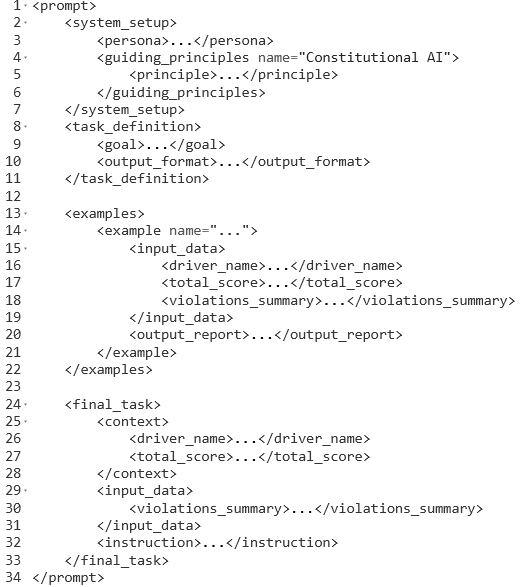
\includegraphics[width=.4\textwidth]{prompt_black_white.png}
\caption{Example structure}
\label{fig:exampleFig1}
\end{figure}

Constructing the prompt for the LLM is central to the system’s success. A function \verb|get_virtual_instructor_prompt_template()| was implemented in the code, which returns a template with multiple sections. This template uses an XML-like structure for clarity. The main sections of the prompt are:

\begin{itemize}
    \item \verb|<system_setup>|: This section establishes the context for the LLM. Within it:
    \begin{itemize}
        \item \verb|<persona>|: Here it is made explicit to the model that it is a “Virtual Driving Instructor, expert in fleet management and telemetry analysis,” with the mission of coaching drivers. This prepares the model to adopt an authoritative yet helpful tone.
        \item \verb|<guiding_principles name="Constitutional AI">|: In this section, four principles that the model must follow are listed. These are effectively the “constitution” for the AI’s responses. In summary, the principles state: (1) Base the feedback strictly on the provided data (avoid assumptions); (2) Maintain a supportive and constructive tone – focus on improvement, not blame, and use respectful language; (3) Give practical, actionable recommendations tied to the events; and (4) Prioritize safety above all, emphasizing accident prevention.
        \item \verb|<task_definition>|: This section explains what is desired from the AI. It specifies the objective (“Generate a driving improvement report...”, i.e., an individual driving performance improvement report) and a description of the output format. The output format is given as a numbered list of sections: (1) General Analysis – greeting and summary with total score; (2) Detailed Improvement Points – explanations of the most significant violations, with risk context and a practical tip for each, including the map link; (3) Final Recommendation – a concluding “golden tip” based on the overall pattern.
    \end{itemize}
    \item \verb|<examples>|: A concrete example is provided within the prompt. Due to prompt length constraints, one example (titled “Analysis for João Silva”) was included. In this example:
    \begin{itemize}
        \item \verb|<input_data>| provides a fictitious driver name “João Silva,” a \verb|total_score| of 85.00, and a \verb|violations_summary| list with one example violation. The listed violation is a speeding event (30 points) with date/time, duration, and a map link.
        \item \verb|<output_report>| provides a sample report corresponding to that input. The content shows how the model is expected to write: it greets João, notes in general terms that some points need attention, then under a subsection “Improvement Points with Context,” it details the speeding violation, including an explanation of the risk, practical tips, and location information. This example is crucial – it demonstrates the desired tone (note it says “Olá, João!” in a friendly manner, and then maintains an encouraging tone) and format (all sections present, sections use appropriately titled Markdown headings, tips are italicized or in list form, etc.). By including this in the prompt, the model has a reference of style and structure to emulate. This is effectively few-shot learning: the model sees one input–output pair (or could see a few) and learns to produce a similar output for new inputs.
    \end{itemize}
    \item \verb|<final_task>|: After the example, the prompt ends with the specific task for the current driver. The real \verb|<driver_name>| and \verb|<total_score>| of the selected driver are then provided, as well as the assembled \verb|<violations_summary>| for that driver (which may have 1–3 main violations). Finally, an \verb|<instruction>| explicitly tells the model to “execute the analysis and generate the report for the specified driver, strictly following the format and guidelines.” This instruction reinforces that it should now apply everything above to produce a new output.
\end{itemize}
The entire prompt is enclosed by a top-level \verb|<prompt>| tag to signal the beginning and end. It was observed that using XML tags (or any distinctive tokens) for each part made it easier to verify or extract sections, if necessary, and likely helps the model differentiate between instruction, example, and data.

\subsection{Autoverification and Post-processing}

After calling the API, the system verifies the response. If the model returns content in the expected structure (which should be Markdown with the sections), the response is accepted. A minimal validation was performed: ensuring that the text is not empty and contains certain keywords that indicate each section is present (for example, “General Analysis,” “Improvement Points,” and “Final Recommendation”). If something is wrong (for instance, the API JSON has no candidates, or the content is not as expected), the code logs an error and returns a message like “Could not generate the analysis.”

Finally, the Markdown report is rendered in the web interface. The user can freely edit it upon review. An Export function was also provided that takes key performance indicators and produces an HTML file for download. The HTML includes, for example, some summary statistics (total events, worst day, etc.) and the generated text. This allows the output to be shared with drivers (for example, via email or text message).

\section{Discussion}

\subsection{Effectiveness of Prompt Engineering in Decision Support Systems}

This project illustrates that careful prompt engineering can transform an LLM viewed as a black box into a domain-specific consultant. By investing effort in the prompt (which acted like a small expert system script), it was possible to achieve model behavior that would otherwise require extensive \textit{fine-tuning} or rule-based programming. The Virtual Instructor effectively encodes a combination of expert knowledge (through the example and principles) and data-driven personalization (through injecting the driver’s actual metrics). This hybrid approach – combining human-written rules (in the prompt) with ML-generated text – proved powerful. It demonstrates a practical way to obtain an explainable AI output without requiring the model to inherently explain its own internal workings.

\subsection{User Acceptance and Trust}

Positive user feedback indicates that explainability tangibly improves user acceptance. Drivers were more willing to engage with feedback when it was in a friendly narrative form. Managers found value in the AI reports as a complement to their own expertise, rather than a replacement. This suggests that AI explanations in the vehicle driving domain can enhance, rather than replace, human judgment when properly designed. The main insight is that the AI serves as a “coaching assistant” that provides structured and consistent feedback, while humans retain the ability to contextualize, modify, and deliver the message personally. This human–AI hybrid approach leverages the strengths of both: the AI’s ability to process large amounts of data and generate consistent explanations, and the human ability to understand the context, build relationships, and adapt communication style.

\section{Conclusion and Future Work}

Several limitations of the current approach suggest directions for future work. First, the prompt engineering approach adopted, while effective, is somewhat fragile – changes in the LLM or API could require adjustments to the prompt. More robust approaches might involve performing \textit{fine-tuning} of a model specifically for this domain. Second, the evaluation conducted was limited to a single dataset and a relatively small user study. A larger-scale deployment would provide more insights into long-term effectiveness and potential behavior change. Third, the current system generates reports for individual drivers, but fleet-level insights and comparative analyses could be valuable. Future work could explore generating fleet-wide reports that identify common patterns and suggest systemic improvements.

Additionally, the system focuses on reactive feedback (analyzing past violations). A more proactive approach could involve real-time \textit{coaching} or predictive analysis to prevent violations before they occur. This would require integration with real-time streams and, possibly, more sophisticated machine learning models for prediction. In sum, this study demonstrated the potential of integrating LLMs aligned to the vehicle telemetry context to improve driving safety and efficiency, although there is room to improve the robustness and scalability of this approach in future developments.

\bibliographystyle{sbc}
\bibliography{sbc-template}

\end{document}